\subsection*{\textbf{2.1 Настройка репозиториев}}
\addcontentsline{toc}{subsection}{2.1 Настройка репозиториев}
\vspace{-0.5cm}

Репозиторий --- это сервер/хранилище, где хранятся пакеты для установки и
обновлений ОС (например, ядра, утилиты и программы). Он может содержать как
бинарные пакеты, так и исходные коды. Репозитории указываются в файле
конфигурации \texttt{/etc/apt/sources.list}. Существуют официальные репозитории
и сторонние, добавлять которые нужно с осторожностью, чтобы избежать
небезопасного ПО.

Бинарные пакеты --- это уже скомпилированные и готовые к установке программы или
утилиты.

Исходные коды --- это текстовые файлы, содержащие программу, которую нужно
скомпилировать в бинарный пакет перед установкой.

Как управлять \texttt{sources.list}: \url{https://wiki.debian.org/SourcesList}

Давайте рассмотрим мой \texttt{/etc/apt/sources.list} в качестве примера.

\begin{center}
\vspace{-0.3cm}
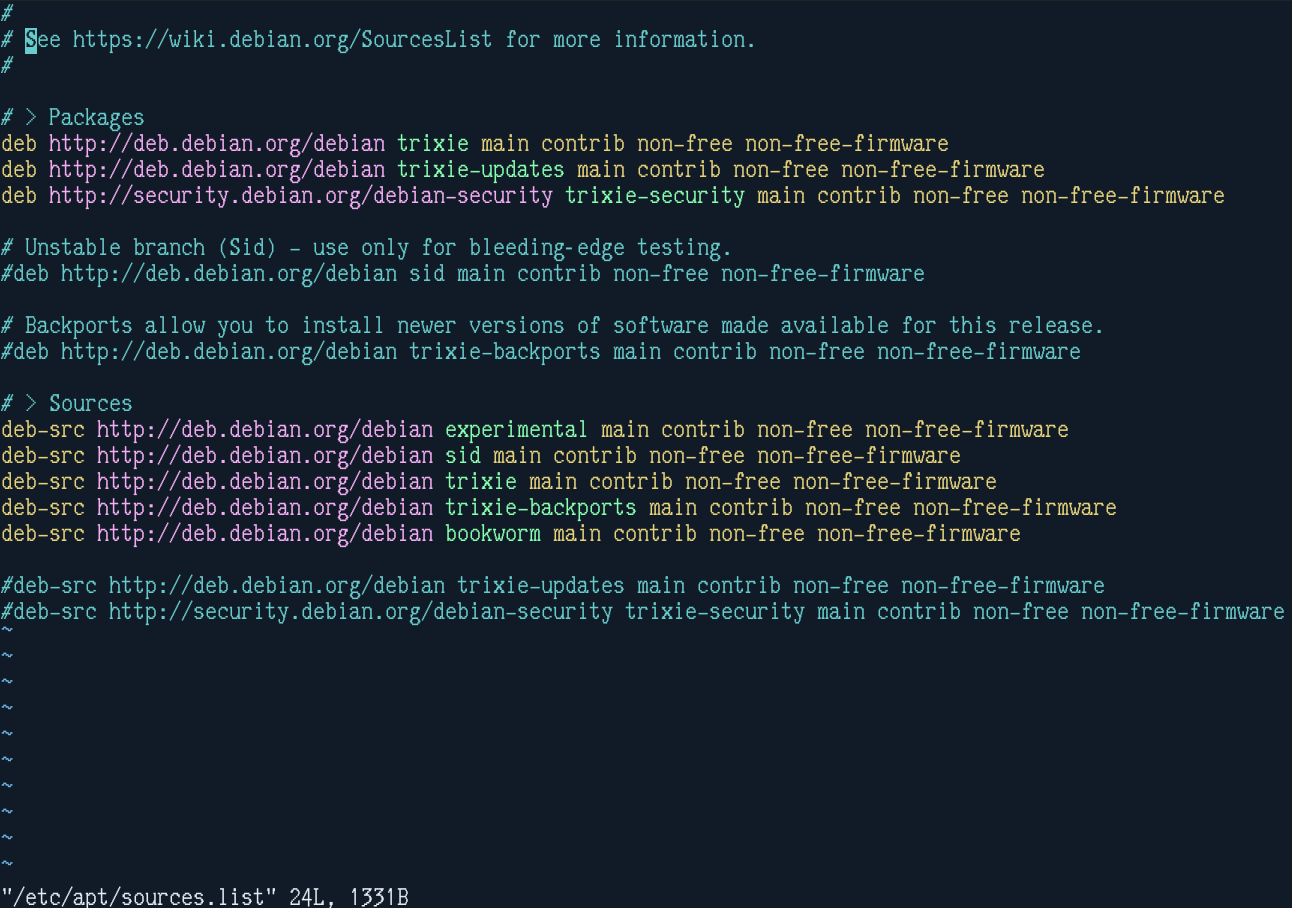
\includegraphics[width=0.95\textwidth]{images/sources-list.png}

\small \textbf{/etc/apt/sources.list}
\vspace{-0.3cm}
\end{center}

\vspace{10cm}

Структура:\\
\texttt{
deb http://site.example.com/debian distribution component1 component2\\
deb-src http://site.example.com/debian distribution component1 component2
}
\vspace{-0.5cm}

\textbf{deb}\\
бинарные пакеты

\textbf{deb-src}\\
пакеты с исходным кодом

\textbf{http://site.example.com/debian}\\
url репозитория

\textbf{distribution}\\
псевдоним релиза, ключевое слово, либо класс релиза

\textbf{component}\\
main, contrib, non-free, non-free-firmware набор пакетов

В секции бинарных пакетов у меня прописаны:\\
\textbf{trixie} основной репозиторий для стабильных пакетов Debian.
\textbf{trixie-updates} репозиторий для обновлений пакетов в основной версии,
включая исправления ошибок и улучшения. \textbf{trixie-security} репозиторий для
обновлений безопасности, содержит патчи и исправления уязвимостей.

В секции исходных пакетов у меня прописаны:\\
\textbf{experimental} содержит экспериментальные версии исходных пакетов,
которые используются для тестирования новых изменений. \textbf{sid} репозиторий
исходников нестабильной ветки Debian, где доступны самые свежие версии пакетов.
\textbf{trixie} исходные пакеты текущего стабильного релиза.
\textbf{trixie-backports} содержит исходники пакетов, перенесённых из более
новых веток для использования в \textbf{trixie}. \textbf{bookworm} исходные
пакеты предыдущего стабильного релиза, которые удобно использовать для сравнения
версий, изменений и сопровождения пакетов между выпусками.

Я прописываю столько секций \textbf{deb-src} только для одного: чтобы сравнивать
изменения и отслеживать их от релиза к релизу. Это нужно не всегда, но иногда
может понадобиться. Для начала работы с Debian достаточно указать свой релиз и
\textbf{sid} (так как мы будем работать с последними версиями пакетов).

\begin{center}
\vspace{-0.3cm}
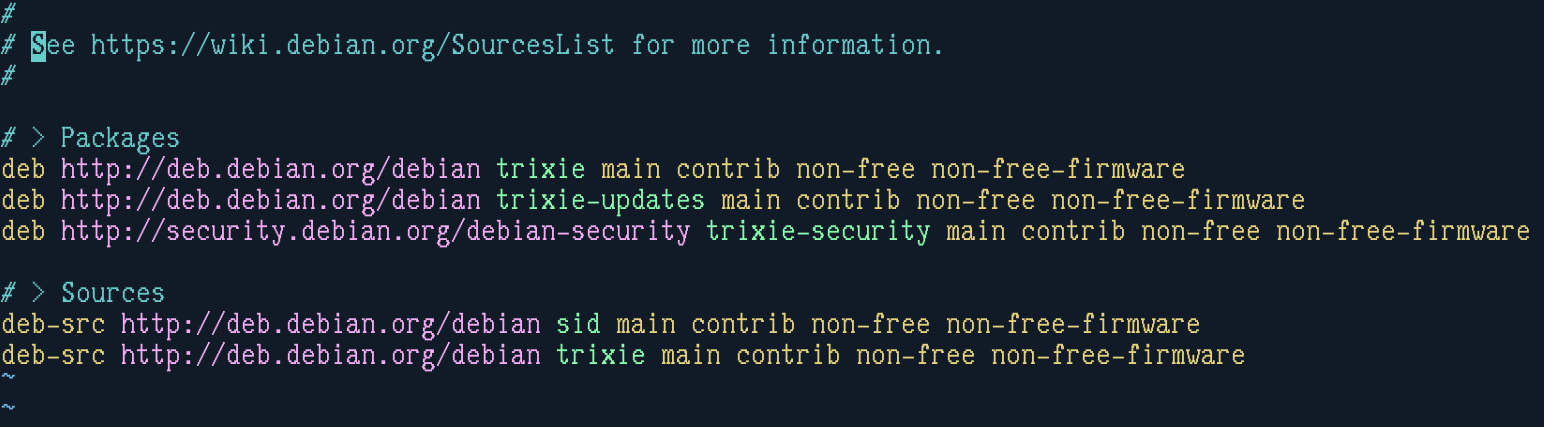
\includegraphics[width=0.95\textwidth]{images/sources-list-clean.png}

\small \textbf{/etc/apt/sources.list}
\vspace{-0.3cm}
\end{center}

\vspace{10cm}

Сделайте:
\vspace{-0.5cm}
\begin{verbatim}
$ apt-get update
\end{verbatim}

\vspace{-0.3cm}
Команда \texttt{apt-get update} обновляет локальный список пакетов, подтягивая
информацию о доступных пакетах и их версиях из репозиториев, указанных в
\texttt{/etc/apt/sources.list}.

После чего можно увидеть доступные версии исходного пакета для скачивания:
\vspace{-0.5cm}
\begin{verbatim}
$ apt-cache madison <package>
\end{verbatim}

\vspace{-0.3cm}
Например:
\vspace{-0.5cm}
\begin{verbatim}
$ apt-cache madison vifm
\end{verbatim}

\begin{center}
\vspace{-0.3cm}
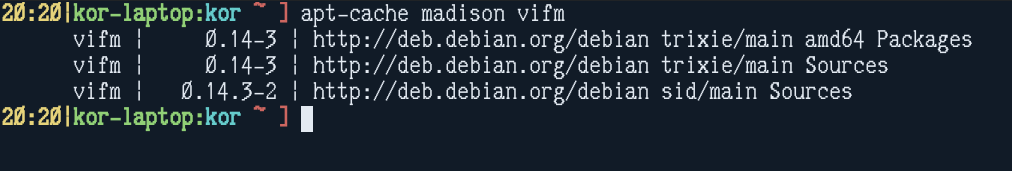
\includegraphics[width=0.95\textwidth]{images/madison-vifm.png}
\vspace{-0.5cm}
\end{center}

\vspace{-0.5cm}
\subsection*{\textbf{2.2 Инструменты и рабочая среда}}
\addcontentsline{toc}{subsection}{2.2 Инструменты и рабочая среда}
\vspace{-0.5cm}

Здесь описаны пакеты и инструменты, которые необходимо установить для базовой
работы с пакетами Debian.

\vspace{-0.5cm}
\begin{verbatim}
$ apt-get install build-essential dpkg-dev devscripts debhelper \
fakeroot lintian autoconf automake libtool dh-make dh-autoreconf \
quilt pbuilder
\end{verbatim}

\vspace{-0.3cm}
Это базовый набор инструментов, необходимый для сборки программ из исходного
кода, подготовки Debian-пакетов, проверки их качества и работы с типичным
autotools-проектом. С его помощью можно собрать программу, оформить её как
Debian-пакет, внести при необходимости патчи и проверить результат на
распространённые ошибки.

Также в список включён инструмент для сборки в чистом изолированном окружении
(pbuilder): он позволяет проверить, что пакет собирается только с указанными
зависимостями и не опирается на пакеты, случайно установленные в основной
системе.

Разработчики и мейнтейнеры Debian в основном собирают пакеты не на своей
основной машине, а в изолированной среде (chroot), чтобы не засорять рабочую
систему лишними зависимостями, устанавливаемыми для сборки, и при этом иметь
возможность проверить, что пакет действительно собирается только с теми
\texttt{Build-Depends}, которые явно указаны в его метаданных.

На практике для этого обычно используют \textbf{pbuilder} (хороший вариант для
начинающих) и \textbf{sbuild} (более распространённое решение для более
продвинутой и регулярной работы).

Важная ссылка: \url{https://wiki.debian.org/pbuilder}

\textbf{pbuilder} и \textbf{sbuild} по сути запускают \textbf{dpkg-buildpackage}
внутри чистого окружения (chroot), добавляя установку \texttt{Build-Depends} и
изоляцию. Это обертки над более низкоуровневыми инструментами.

Чтобы понять, из каких этапов состоит сборка, выполняемая
\textbf{dpkg-buildpackage}, можно обратиться к документации:
\url{https://man7.org/linux/man-pages/man1/dpkg-buildpackage.1.html}

Например, в Debian для автоматической сборки пакетов используется сеть
\textbf{buildd}-серверов. Исходные пакеты собираются в изолированных окружениях
с помощью \textbf{sbuild} и связанных с ним инструментов.

Сеть автоматической сборки: \url{https://www.debian.org/devel/buildd/}

Debian Package Auto-Building: \url{https://buildd.debian.org/}

Например, давайте посмотрим страницу \textbf{buildd} со статусом сборки пакета
vifm на разных архитектурах Debian:
\url{https://buildd.debian.org/status/package.php?p=vifm&suite=sid}

\vspace{-0.5cm}
\subsection*{\textbf{2.3 Структура исходного пакета}}
\addcontentsline{toc}{subsection}{2.3 Структура исходного пакета}
\vspace{-0.5cm}

Теперь мы готовы скачать исходный пакет
\href{https://tracker.debian.org/pkg/vifm}{vifm} и посмотреть его содержимое.
Обычно я перехожу во временную директорию \texttt{/tmp} и работаю там.
\vspace{-0.5cm}
\begin{verbatim}
$ apt-get source vifm # скачается самая последняя версия
\end{verbatim}

\vspace{-0.3cm}
Или скачать исходный пакет определенной версии:
\vspace{-0.5cm}
\begin{verbatim}
$ apt-get source vifm=0.14-3 # скачается версия из trixie
\end{verbatim}

\vspace{-0.3cm}
Исходный пакет будет скачан из репозитория Debian по адресу\\
\url{http://deb.debian.org/debian} (из соответствующей ветки/дистрибутива).


И так, мы имеем исходный пакет (source package):
\begin{center}
\vspace{-0.3cm}
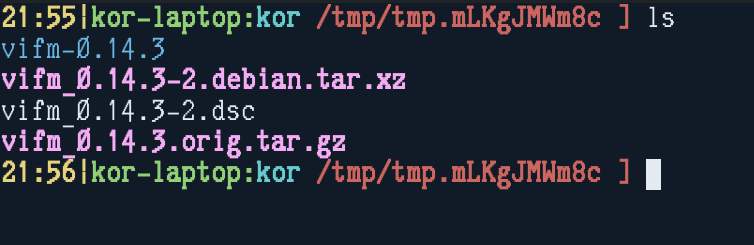
\includegraphics[width=0.95\textwidth]{images/source-package.png}
\end{center}

\vspace{10cm}

\textbf{vifm\_0.14.3.orig.tar.gz}\\
Оригинальные исходные файлы программы без изменений. Другими словами, это
неизмененные upstream-файлы от оригинальных авторов.

\textbf{vifm\_0.14.3-2.dsc}\\
Описание исходного пакета, где указана версия и ссылка на исходники. Этот файл
обычно подписывается сопровождающим пакета (подлинность).

\textbf{vifm\_0.14.3-2.debian.tar.xz}\\
Патчи и изменения для Debian (изменения в пакете, специфичные для Debian).

\textbf{vifm-0.14.3}\\
Директория, куда распаковываются файлы пакета.

Форматы файлов исходного пакета Debian могут различаться от пакета к пакету:
например, оригинальные исходные файлы и Debian-изменения могут быть упакованы в
архивы \textbf{.tar.gz}, \textbf{.tar.xz} или \textbf{.tar.bz2}, в зависимости
от выбранного способа сжатия. Поэтому набор файлов и их расширения не всегда
одинаковы, хотя их назначение остается тем же. Формат сжатия выбирает maintainer
пакета.

Давайте перейдем в директорию с исходными файлами пакета и посмотрим, что там:

\begin{center}
\vspace{-0.3cm}
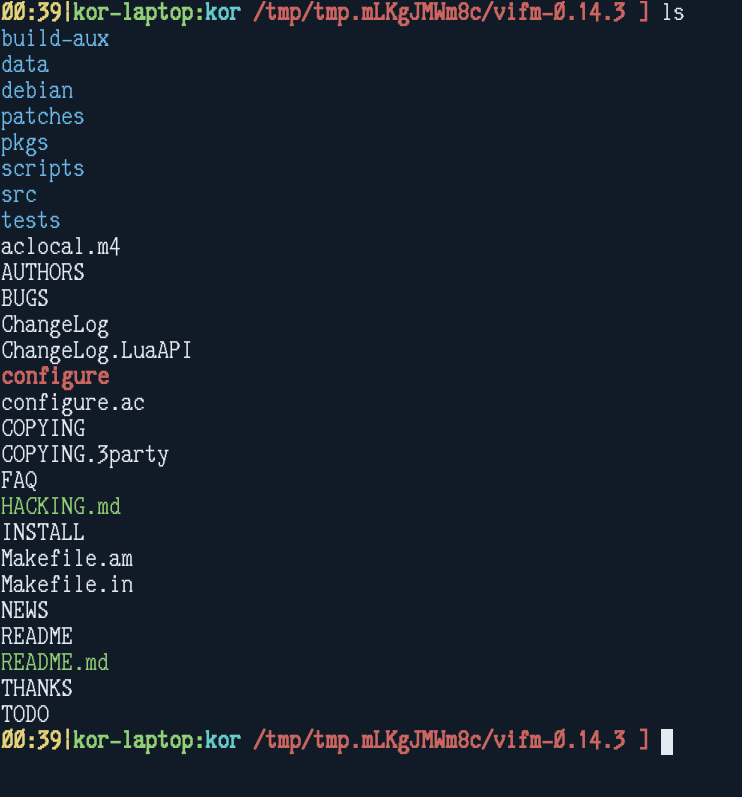
\includegraphics[width=0.70\textwidth]{images/source-files.png}
\end{center}

\vspace{10cm}

Если говорить просто, то перед нами исходное дерево проекта vifm. Сопровождающий
пакета взял исходные файлы из репозитория \url{https://github.com/vifm/vifm} и
импортировал их в Debian. На ранних этапах я бы не советовал слишком глубоко в
них погружаться, так как в структуре проекта легко потеряться.

Наличие файлов configure, configure.ac, Makefile.am, Makefile.in и aclocal.m4
показывает, что проект использует систему сборки Autotools. В дереве проекта
присутствуют исходный код, тесты, скрипты, данные и директория \textbf{debian/},
которая для нас наиболее важна.

Разработчики и мейнтейнеры Debian в основном работают с файлами в директории
\textbf{debian/}, где хранятся конфигурации для сборки пакета, патчи и другие
специфичные для Debian файлы. Им нужно гарантировать, чтобы программное
обеспечение успешно собиралось, правильно интегрировалось с системой и корректно
устанавливалось на всех поддерживаемых версиях Debian. Для этого они проверяют
совместимость, управляют зависимостями и обеспечивают соблюдение стандартов
качества, установленных для Debian-пакетов.

Я не буду здесь подробно останавливаться на назначении всех файлов, которые
могут встречаться в этой директории, поскольку для этого лучше обратиться к
руководствам из главы \textbf{Введение}, в частности к материалам
\textbf{среднего} уровня. Вместо этого предлагаю сосредоточиться на базовых
конфигурационных файлах на примере пакета
\href{https://tracker.debian.org/pkg/vifm}{vifm}.

\begin{center}
\vspace{-0.3cm}
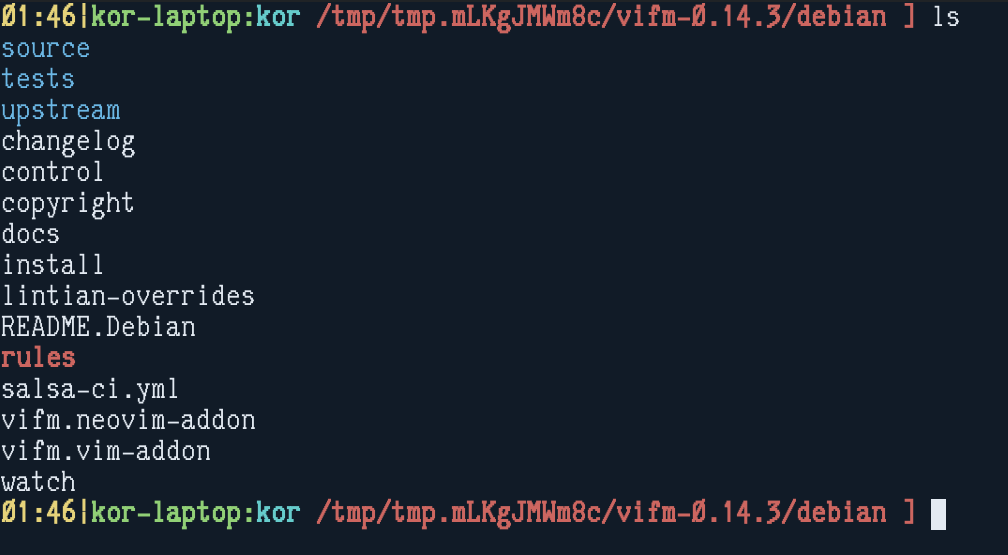
\includegraphics[width=0.95\textwidth]{images/debian-files.png}
\end{center}

\textbf{source}\\
Директория, содержащая дополнительные файлы, специфичные для сборки исходного
пакета.

\textbf{source/format}\\
Файл, указывающий формат исходного пакета, например, 3.0 (quilt).

\vspace{10cm}

\textbf{tests}\\
Директория с тестами, которые проверяют работоспособность пакета после установки
(autopkgtest).

\textbf{tests/control}\\
Конфигурационный файл для тестов, описывающий, какие тесты и как должны быть
выполнены.

\textbf{upstream}\\
Содержит информацию об исходных файлах проекта.

\textbf{upstream/metadata}\\
Upstream ссылки.

\textbf{changelog}\\
История изменений пакета с датами и описанием изменений в каждой версии.

\textbf{control}\\
Описание пакета, включая его название, описание, зависимости, версии и прочее.

\textbf{copyright}\\
Лицензионная информация о пакете, включая авторские права и условия
распространения.

\textbf{docs}\\
Директория с документацией, связанной с пакетом.

\textbf{install}\\
Файл, в котором перечисляют файлы и каталоги, которые нужно установить в пакет
при его сборке, а также куда именно их поместить.

\textbf{lintian-overrides}\\
Файл, в котором можно переопределить предупреждения и ошибки, генерируемые
инструментом
\href{https://manpages.debian.org/testing/lintian/lintian.1.en.html}{lintian}
при проверке пакета.

\textbf{README.Debian}\\
Документация, специфичная для Debian.

\textbf{rules}\\
Основной скрипт для сборки пакета, который описывает, какие команды и шаги нужно
выполнить для компиляции и упаковки пакета. Тут пригодятся знания Makefile.

\textbf{salsa-ci.yml}\\
Конфигурация для CI/CD (непрерывной интеграции), специфичная для платформы Salsa
(GitLab Debian). Можно посмотреть, как это работает на практике
\url{https://salsa.debian.org/debian/vifm/-/pipelines}

\textbf{watch}\\
Файл, который указывает, где можно отслеживать обновления исходного кода пакета.
Чаще всего это GitHub.

Подробно изучите каждый файл, особенно \textbf{control} и \textbf{rules}. Если
вас интересует, что значит каждое поле в \textbf{control}, можно полистать
\url{https://www.debian.org/doc/debian-policy/ch-controlfields.html}.

Структура пакетов Debian в целом единообразна, поэтому при работе с ними быстро
привыкаешь к принятым стандартам. В Debian большое значение придаётся правилам
оформления пакетов. Их соблюдение обеспечивает аккуратную структуру пакета,
корректную интеграцию в систему, а также совместимость, удобство установки и
последующего обновления. Поэтому желательно знать
\href{https://www.debian.org/doc/debian-policy/}{Debian Policy} --- не целиком,
но хотя бы в основных моментах.
